% !TEX root = main.tex
\documentclass[a4paper, UKenglish, 11pt]{uiomaster}
\usepackage{lipsum}
\usepackage[subpreambles=true]{standalone}
\usepackage[table,xcdraw]{xcolor}

\begin{document}

\chapter{Localizing Single Current Dipole Sources} \label{chap:simple_dipole_FFNN}
\rednote{Figure texts not fixed jet}
In this chapter, we will delve into the performance of the fully connected feed-forward neural network (FCNN) in solving the inverse problem. Our primary focus centers on investigating whether the accuracy of the neural network can be linked to the precise positioning and orientation of the current dipoles it is tasked with identifying or if the performance remains consistent across all brain regions and structures. Moreover, we shall employ a range of diverse error metrics to rigorously evaluate the performance of the network in this task.


\section{EEG Sensitivity of Dipole Location and Orientation}
According to Ness et al. (2021) \cite{naess2021biophysically}, EEG signals demonstrate limited sensitivity to minor shifts in the precise location of neural current dipoles. This insensitivity can be attributed to the considerable separation between EEG electrodes and cortical neural sources compared to the dimensions of individual neurons and the thickness of the human cortex. Before evaluating the overall performance of our network, our investigation seeks to ascertain whether neighboring neural dipoles yield nearly indistinguishable EEG signals or exhibit noticeable distinctions. This exploration provides valuable insights into the network's ability to handle the complexity of the problem. If two dipoles located only 1 mm apart yield nearly identical results, it signifies a commendable performance by the network if it ables to distinguish at this scale. We emphasize that  in this context, ''neighboring'' is defined based on the resolution of the NYHM. To assess the similarity in EEG signals between nearby dipoles, we employ the Pearson correlation coefficient.

The Pearson correlation coefficient is a statistical measure that quantifies the relationship between two variables. It is defined as the ratio of the covariance of the two variables to the product of their standard deviations. The coefficient ranges from -1 to 1, with -1 denoting a perfect negative correlation and 1 indicating a perfect positive correlation. A coefficient of 0 signifies the absence of a linear relationship between the variables \cite{numpy-docs}.

In Figure \ref{fig:neighbour_dipoles}, we present EEG signals corresponding to dipoles located in close proximity within the New York Head Model's cortical matrix. The upper panel illustrates the two distinct EEG signals originating from the blue and green dipoles, while the lower panel shows the EEG signal corresponding to the blue and red dipoles. The blue central dipole is positioned between the green and red dipoles, located at the leftmost and rightmost positions in the NYHM cortical matrix, respectively. The Euclidean distance between the blue and green dipoles is 0.914 mm, while the blue and red dipoles are separated by 1.926 mm.

In Figure \ref{fig:neighbour_dipoles}, the EEG signals of the blue and green dipoles exhibit significant overlap, with a high correlation coefficient of 0.966, indicating a strong positive relationship. In contrast, the EEG signals of the blue and red dipoles show less resemblance, with a correlation coefficient of 0.695, indicating a weaker linear relationship.

The observed variability in the correlation between the EEG signals of neighboring dipoles can be attributed to differences in the orientation of their respective dipole's normal vectors. The observed smaller value in the correlation matrix between the red and blue dipole, in contrast to the higher correlation between the blue and green dipole, is related to the more pronounced angular disparity in the normal vector alignment between the red dipole and the blue dipole. In contrast, there is a relatively smaller angular difference observed between the green dipole's normal vector and that of the blue dipole.

The distinct differences in the orientation of normal vectors arise from constraints imposed during data generation, which are designed to ensure that dipole orientations remain perpendicular to the complex folding of the cerebral cortex. As a result, neighboring dipoles within the NYHM possess distinct normal vectors, potentially leading to significantly different simulated EEG signals.

Furthermore, it is important to note that the separation between the red dipole and the blue dipole is somewhat greater than the distance between the blue and green dipoles. This variation in separation can be attributed to the specific construction of the NYHM cortex, as established by its developers.

In conclusion, these findings underscore the intricate nature of EEG signals, where the correlation analysis reveals varying degrees of similarity for neighboring dipoles. In some scenarios, it becomes evident that the linear relationship between EEG signals originating from distinct dipoles is relatively small, suggesting the network's capability to separate the EEG signals. In other instances, the EEG signals exhibit significant similarity, which may pose a challenge for the network in distinguishing them.


%Despite the common belief that neurons in the upper cortical layers would dominate the EEG due to their proximity to the electrode compared to neurons in deeper layers, such location differences do not significantly affect the EEG signals. This phenomenon can be explained by the fact that the low conductivity of the skull introduces a spatial low-pass filtering effect, which mitigates the impact of location discrepancies.
% Maybe what is meant here is that we therefore only consider the outer corical surface

\begin{figure}[!htb]
    \centering
    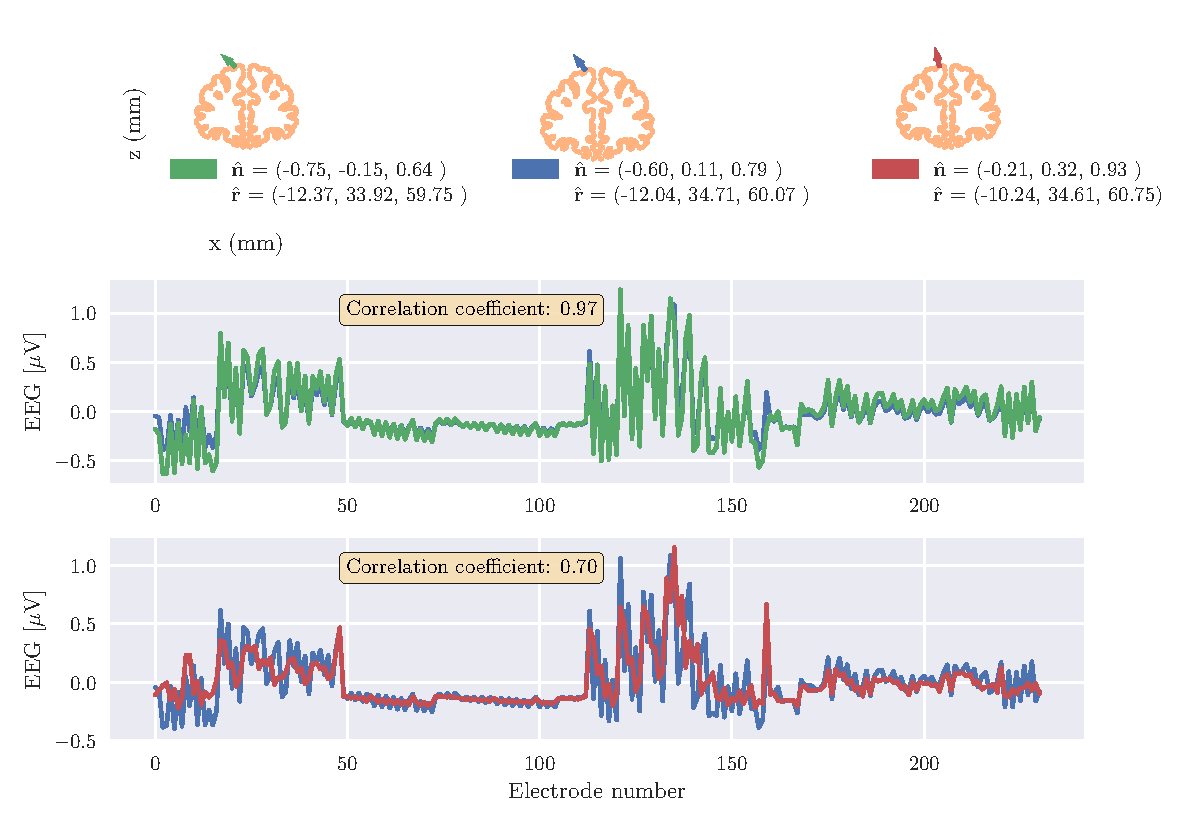
\includegraphics[width=\linewidth]{figures/compare_dipoles.pdf}
    \caption{EEG signals plotted against electrode number for three neighbouring dipoles with normal vectors (-0.60, 0.11, 0.79), (-0.75, -0.15, 0.64), (-0.21, 0.32, 0.93) and positions (-12.04, 34.71, 60.07), (-12.37, 33.92, 59.75), (-10.24, 34.61, 60.75). The correlation coefficient between the blue and green dipole is 0.97, while it is 0.70 for the blue and red dipole. \rednote{Which coordinate system? Where is (0,0,0) located?}}
    \label{fig:neighbour_dipoles}
\end{figure}

\FloatBarrier

\section{Performance Evaluation} \label{sec:performace_evaluatoin}
\rednote{Move to training chapter?}
Based on the findings of Akalin Acar and Makeig 2013 \cite{akalin2013effects} and Biasiucci et al. 2019 \cite{biasiucci2019electroencephalography}, source localization using spherical head models typically yields localization errors in the range of 10-30 mm. On the other hand, the utilization of modern subject-specific head models is expected to result in errors of less than 10 mm. The New York Head Model falls within the second category, and we will, therefore, let 10 mm serve as our guideline when evaluating the network's predictions.

Nevertheless, we emphasize that our primary objective is not necessarily the development of a flawless neural network for immediate clinical applications. Our aim is to ascertain whether a simple fully connected feed-forward neural network can effectively discern patterns and approximate dipole positions based on the simulated EEG data, collected using LFPy and the integrated Head Model, as outlined in Chapter 3.

Within this section, we will employ various techniques to assess the network's performance. This evaluation will include tracking the loss during training, utilizing different sets of error metrics to calculate the average prediction error, and determining the distribution of test samples falling within predefined threshold values.

\subsection{Results from Training and Validation Process}
The FCNN underwent 500 epochs of training, and the convergence of the mean Euclidean distance (MED) is illustrated in Figure \ref{fig:single_dipole_accuracy}. The entire training process, encompassing data loading and preprocessing, took approximately 1.5 hours, with each epoch having an average training duration of about 11.00 seconds.

The validation loss exhibited a noticeable stabilization trend after approximately 350 epochs. At this point, the training could have been terminated. However, we chose to continue training for the full 500 epochs to confirm that no further improvements in validation data performance were attainable and to emphasize the network's full convergence.

Figure \ref{fig:single_dipole_accuracy} visually demonstrates a clear reduction in loss, indicating the network's effective learning of patterns in the data. Validation loss stabilization becomes evident around the 350-epoch mark, while the training loss continues to decrease until it stabilizes between 400 and 500 epochs. This observation suggests that the model did not demonstrate signs of overfitting, as the validation loss remained constant, and the training loss ultimately stabilized. At epoch 500, the MED training loss is equal to 0.317 mm, while the MED validation loss measures 1.781 mm.

Furthermore, Figure \ref{fig:single_dipole_accuracy_targets} offers insight into the evolution of validation loss for the individual target coordinates—$x$, $y$, and $z$—as plotted against training epochs. This figure reaffirms that all three target coordinates were equally weighted, resulting in somewhat similar loss values for each. Additionally, it illustrates that the minor fluctuations in loss observed before 350 epochs disappear beyond this threshold, indicating a stable loss for all three target coordinates. This observation aligns with the trend of validation loss stabilization observed at approximately 350 epochs, as shown in Figure \ref{fig:single_dipole_accuracy}.

\begin{figure}[!htb]
    \centering
    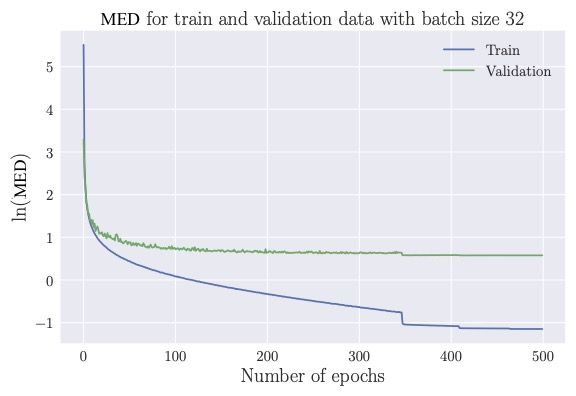
\includegraphics[width=\linewidth]{figures/Simple/new_loss.jpg}
    \caption{Training- and validation MED loss for the fully connected feed-forward (FCNN) neural network with 50,000 samples.}
    \label{fig:single_dipole_accuracy}
\end{figure}

\begin{figure}[!htb]
    \centering
    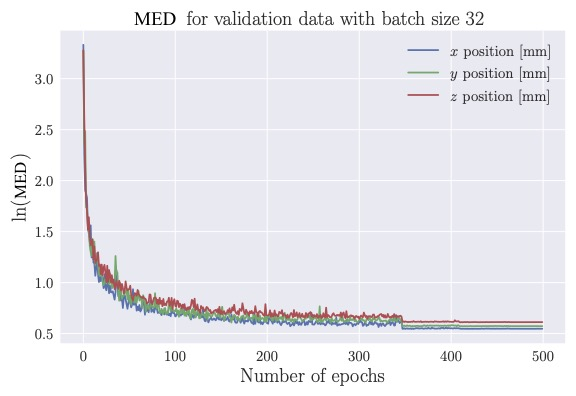
\includegraphics[width=\linewidth]{figures/Simple/new_target.jpg}
    \caption{Validation MED loss for the separate target values; the $x$-, $y$-, $z$-coordinate.}
    \label{fig:single_dipole_accuracy_targets}
\end{figure}


\subsection{Testing Methodology and Accuracy}
\rednote{Move to training chapter?}
% We begin by introducing the standard inverse problem for our neural network, DiLoc. In this context, the standard inverse problem refers to the task of predicting the x-, y-, and z-coordinates of dipole current sources responsible for generating measured EEG signals. The goal is to feed the network with EEG data corresponding to the electrical activity from randomly distributed dipoles in the cerebral cortex and have the network accurately output the locations of these current dipoles.
%For this specific problem, the network demonstrates remarkable performance even without the use of L1 regularization. However, we include L2 penalty with a value of 0.5 to promote more generalizable solutions.
Upon achieving full training convergence, a neural network demonstrates its capacity to discern essential patterns within the training data set, optimizing its parameters to minimize the cost function. To further assess the performance of the FCNN, our attention turns to an independent test data set, comprising 20,000 samples. This data set remains entirely shielded from the network during the training process, serving as an unbiased and objective gauge of the model's predictive accuracy and its ability to generalize effectively to novel, unseen data.

In order to comprehensively evaluate the neural network's performance on the untouched test data set and ensure the comparability of our results with other models, we employ a diverse set of error metrics. In addition to the primary metric of mean Euclidean distance used for assessing the accuracy of the network's predictions regarding the positions of current dipoles in the cerebral cortex, utilizing the metrics of Mean Absolute Error (MAE), Mean Squared Error (MSE) and Root Mean Squared Error (RMSE) are utilized in order to evaluating the network's performance with respect to distinct target coordinates. This approach enables us to discern whether the network faces greater challenges in predicting one dimension over others or if it consistently maintains a uniform level of performance across all coordinate dimensions.

The MAE metric provides a direct measure of the magnitude of the difference between predicted coordinates ($x$, $y$, or $z$) and their true values. MAE offers a straightforward and easily interpretable indicator of the model's prediction accuracy for each dimension. It allows us to ascertain whether the network consistently delivers precise predictions for all target values or whether variations in accuracy manifest across different coordinate dimensions.

The MSE on its side introduces a squaring process that significantly penalizes larger errors. MSE measures the variance of residuals in squared units. While this feature emphasizes and addresses substantial error spread within the predictions, it does present values in squared units of the target values. This can pose a challenge when assessing individual coordinate components.

To mitigate the squared unit issue associated with MSE while still considering error spread, RMSE is included in the evaluation framework. RMSE measures the standard deviation of residuals, balancing the emphasis on significant errors while presenting results in units that align with the target coordinate values.

Both MSE and RMSE exhibit a higher sensitivity to larger errors, as they penalize substantial deviations more strongly when calculating the average squared differences between predicted and actual values. This contrasts with the MAE metric, which treats all errors, regardless of size, on an equal footing. Consequently, a high MSE or RMSE signifies a more extensive error spread, wherein predictions substantially deviate from the true values. Conversely, a lower MSE or RMSE indicates that prediction errors are less dispersed, and most predictions closely align with the true values. Smaller MSE and RMSE values signify a superior model fit and lower prediction error.


\subsubsection{Position Spesific Performance}
The MED between the network's predictions on the unseen test data and the true target values measures 1.33 mm. It is worth noting that this error is smaller than the one observed in the validation data, mainly due to the absence of noise in the test data. This high level of precision is further exemplified by the statistics presented in Table \ref{table:MED}. All predictions for the test samples exhibit an Euclidean distance of less than 15 mm, signifying a consistently high level of accuracy. Furthermore, an impressive 99.995$\%$ of the predictions fall within an Euclidean distance of less than 10 mm, and 97.753$\%$ of the predictions achieve an Euclidean distance of less than 5 mm. This numbers indicate a notably high degree of precision.

\begin{table}[]
  \centering
\begin{tabular}{|ccc|}
\hline
\rowcolor[HTML]{CBCEFB}
\multicolumn{3}{|c|}{\cellcolor[HTML]{CBCEFB}\textbf{Euclidian Distance for Test Samples}}                                                             \\ \hline
\rowcolor[HTML]{EFEFEF}
\multicolumn{1}{|c|}{\cellcolor[HTML]{EFEFEF}ED \textless 5 mm} & \multicolumn{1}{c|}{\cellcolor[HTML]{EFEFEF}ED \textless 10 mm} & ED \textless 15 mm \\ \hline
\rowcolor[HTML]{FFFFFF}
\multicolumn{1}{|c|}{\cellcolor[HTML]{FFFFFF}99.735 $\%$}       & \multicolumn{1}{c|}{\cellcolor[HTML]{FFFFFF}99.995 $\%$}        & 100$\%$        \\ \hline
\end{tabular}
\caption{\textbf{ED between targets and predictions of test samples; Predicting Single Dipole Location with a FFNN} \newline
Performance of the network on the test data set comprising 20,000 samples, presented as the percentage of samples falling within ED thresholds of 5 mm, 10 mm and 15 mm respectively.}
\label{table:MED}
\end{table}

Table \ref{table:error_simple_dipole} displays the results for various error metrics corresponding to the network's predictions. Beginning with the MAE values for the $x$, $y$, and $z$-coordinates, we observe results ranging from 0.645 mm to 0.678 mm. These findings indicate that, on average, the network's predictions exhibit errors smaller than 1 mm in each coordinate.

The MSE values range from 0.747 mm$^2$ to 0.824 mm$^2$. The smaller MSE values signify high performance, with all values comfortably below a 1 mm$^2$ threshold. This finding indicate minimal error spread and few significant deviations between predicted and true coordinates.

RMSE values range from 0.864 mm to 0.908 mm. It is important to note that RMSE is slightly higher than the corresponding MSE values due to the square root operation involved. However, all RMSE values remain below the 1 mm threshold, signifying that the predictions maintain a limited error spread, typically staying within 1 millimeter of the actual values.

% Additionally, the $z$-coordinate's smaller representation compared to the $x$- and $y$-coordinates could contribute to the consistently larger errors in the $z$-direction.
%One plausible explanation is related to the nature of the inverse problem, where the depth of the dipole sources primarily influences the magnitude rather than the pattern of EEG recordings. However, we underscore that this discrepancy in error magnitude is very small and could also be influenced by randomness.

For an assessment of overall positional errors, the table holds the averaged Mean Absolute Error (MAE), Mean Squared Error (MSE), and Root Mean Squared Error (RMSE) across the three spatial coordinates. The resulting error values reveal minimal deviations, yielding a total MAE of 0.662 mm, a total MSE of 0.782 mm$^2$, and a total RMSE of 0.884 mm. Notably, among the three coordinates, the $z$-coordinate exhibits the highest errors accross all metrics. This observation suggests that the network might encounter somewhat greater challenges in accurately predicting the $z$-coordinate of the dipole source.

% Please add the following required packages to your document preamble:
% \usepackage[table,xcdraw]{xcolor}
% If you use beamer only pass "xcolor=table" option, i.e. \documentclass[xcolor=table]{beamer}
\begin{table}[!htb]
\begin{tabular}{l|cccc|}
\cline{2-5}
\rowcolor[HTML]{CBCEFB}
\cellcolor[HTML]{FFFFFF}                           & \multicolumn{4}{c|}{\cellcolor[HTML]{CBCEFB}{\color[HTML]{000000} \textbf{Error Metrics for Target Values}}}                                                                                                                                                                                                                                                                                                                                                     \\ \cline{2-5}
\rowcolor[HTML]{EFEFEF}
\cellcolor[HTML]{FFFFFF}\textbf{}                  & \multicolumn{1}{l|}{\cellcolor[HTML]{EFEFEF}\begin{tabular}[c]{@{}l@{}}x-coordinate\\ {[}mm{]}\end{tabular}} & \multicolumn{1}{l|}{\cellcolor[HTML]{EFEFEF}\begin{tabular}[c]{@{}l@{}}y-coordinate \\ {[}mm{]}\end{tabular}} & \multicolumn{1}{l|}{\cellcolor[HTML]{EFEFEF}\begin{tabular}[c]{@{}l@{}}z-coordinate \\ {[}mm{]}\end{tabular}} & \multicolumn{1}{l|}{\cellcolor[HTML]{EFEFEF}\begin{tabular}[c]{@{}l@{}}Position \\ Error {[}mm{]}\end{tabular}} \\ \hline
\multicolumn{1}{|l|}{\cellcolor[HTML]{EFEFEF}MAE}  & \multicolumn{1}{c|}{0.645}                                                                                  & \multicolumn{1}{c|}{0.665}                                                                                   & \multicolumn{1}{c|}{0.678}                                                                                   & 0.662                                                                                                              \\ \hline
\multicolumn{1}{|l|}{\cellcolor[HTML]{EFEFEF}MSE}  & \multicolumn{1}{c|}{0.747}                                                                                  & \multicolumn{1}{c|}{0.775}                                                                                   & \multicolumn{1}{c|}{0.824}                                                                                   & 0.782                                                                                                              \\ \hline
\multicolumn{1}{|l|}{\cellcolor[HTML]{EFEFEF}RMSE} & \multicolumn{1}{c|}{0.864}                                                                                  & \multicolumn{1}{c|}{0.880}                                                                                   & \multicolumn{1}{c|}{0.908}                                                                                   & 0.884                                                                                                              \\ \hline
\end{tabular}
\caption{\textbf{Evaluation of the FFNN performance utilizing different Error Metrics.} \newline
FFNN performance on test data set consisting of 20,000 samples. The errors are measured using Mean Squared Error (MSE), Mean Absolute Error (MAE), and Root Mean Squared Error (RMSE).}
\label{table:error_simple_dipole}
\end{table}

To further demonstrate the network's performance, we examine a randomly selected sample from the test data set. For a dipole located at x = 66.5 mm, y = -26.4 mm, and z = 41.9 mm, the network predicts the coordinates to be $\tilde{x}$ = 66.9 mm, $\tilde{y}$ = -26.1 mm, and $\tilde{z}$ = 41.7 mm. The predicted values closely align with the true values, exhibiting a minimal error of 0.4 mm in the $x$-coordinate, 0.3 mm in the $y$-coordinate, and 0.2 mm in the $z$-coordinate, resulting in a total Euclidean distance of 0.54 mm. In Figure \ref{fig:prediction_FFNN_example}, we have illustrated the network's predicted position $\mathbf{r}$ of the dipole alongside the target position $\mathbf{\tilde{r}}$.

\begin{figure}
  \hspace*{-10cm}
  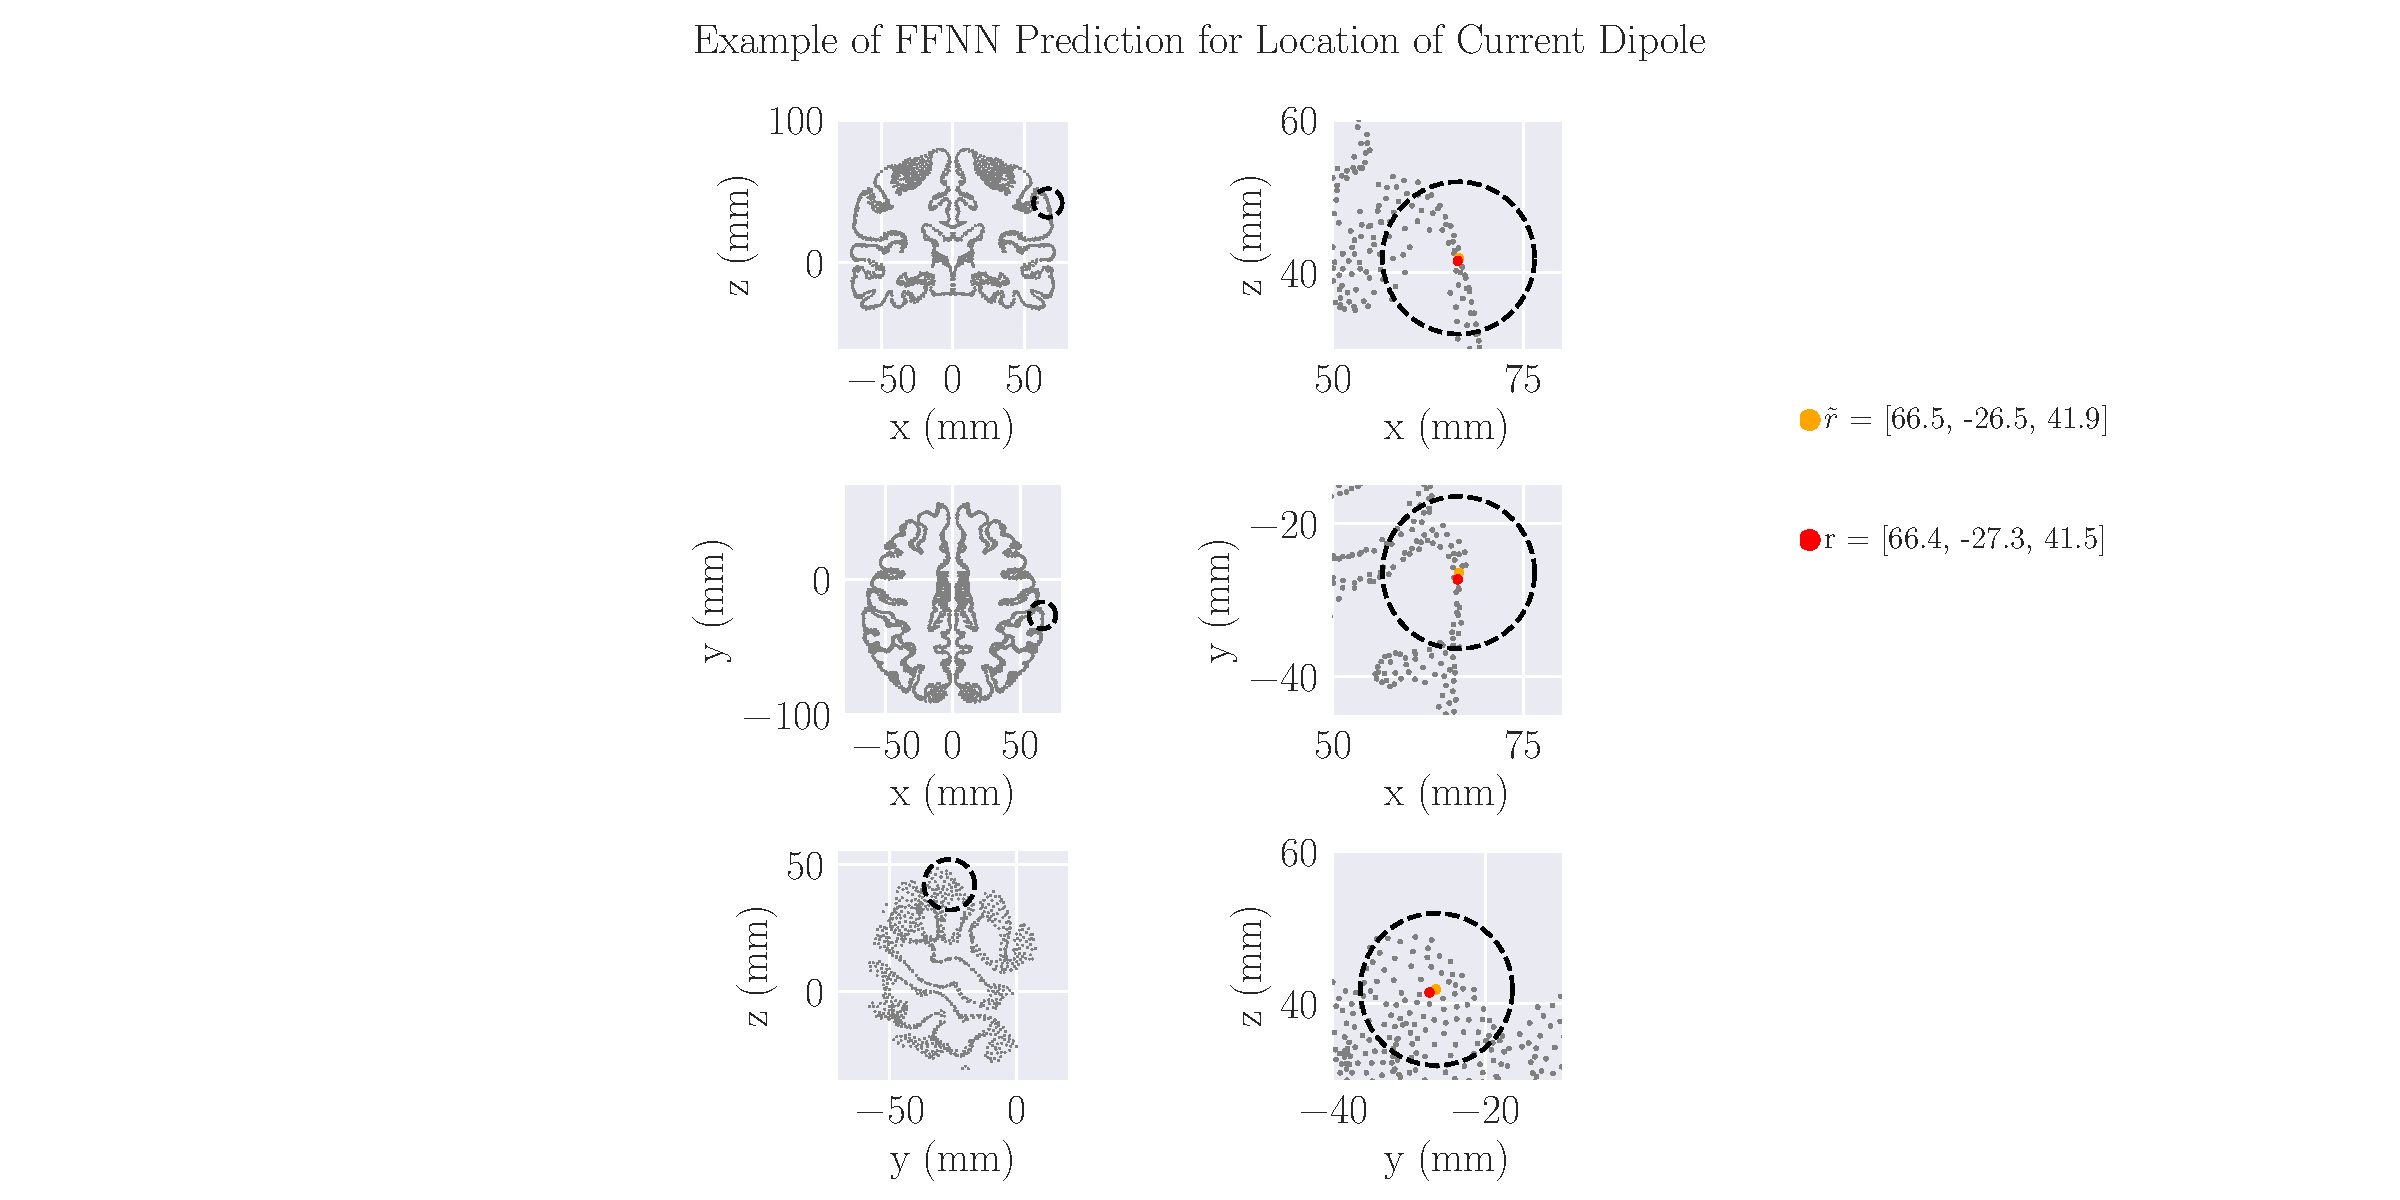
\includegraphics[width=28cm]{figures/FFNN_single_dipole_prediction.pdf}
  \caption{The networks predicted position $r$ of a dipole within the test data set and the target position $\tilde{r}$. The target dipole is marked in orange and the predicted position is marked by a red dot.}
  \label{fig:prediction_FFNN_example}
\end{figure}

\subsection{Performance at Different Brain Structures}

Figure \ref{fig:MED_crossections} presents the distribution of Euclidean Distances for various dipole locations within the New York head model cortex matrix. The figure offers valuable insights into the spread of errors across different regions of the cortex, with three cross-sections—front, top, and side—provided for examination. It is important to note that these cross-sections unavoidably include data points from the training, validation, and test data sets, making these results indicative of the network's overall performance rather than real-world scenarios. However, the analysis aims to examine the distribution of errors and identify potential areas where the network's performance may be weaker, helping to gain valuable insights into its predictive capabilities.

The Euclidean Distance (ED) values presented in the panels are mostly below 1 mm, which indicates a high level of accuracy in the network's predictions. These results are promising and demonstrate the network's ability to estimate dipole locations with a high level of precision. The panels also provide an opportunity to evaluate whether the network exhibits differential performance for dipoles located in a gyrus as opposed to those in a sulcus.

Initially, it might be assumed that EEG signals originating from dipoles in the sulcus present greater challenges for the network's analysis and prediction. This assumption is based on the deeper placement of dipoles within a sulcus compared to those in a gyrus, as well as the potential complexities introduced by the dipole's orientation within the cortex. However, upon closer examination of Figure \ref{fig:MED_crossections}, it becomes evident that the distribution of ED values does not exhibit a clear correlation with the brain's structural characteristics. The ED values seem to vary across different regions, suggesting that the network's performance is not notably affected by the differentiation between gyri and sulci. Surprisingly, the Mean Euclidean Distance for all data points where dipoles are located in a sulcus is measured to be 1.68 mm, which is even smaller than for dipoles in a gyrus, where the Mean Squared Error measures 1.70 mm. This observation further challenges the initial assumption and indicates that the network demonstrates exceptional accuracy in predicting dipole locations, irrespective of their placement within the cortex.

%These relatively small MED values further underscore the network's remarkable capacity to effectively capture the intricate features within the human brain across different cortical structures. features and variations associated with deeper cortical placements. These findings not only attest to the network's robustness but also reinforce its potential for precise dipole localization within the human brain across different cortical structures.

\rednote{Is this considered "theory" and should be mentioned earlier?}
\rednote{FIX MORE}
Further, the panels reveal a slightly higher concentration of data points with red marks in the deeper locations within the cortex, indicating higher ED values. This observation is consistent with the slightly higher error values observed for the $z$-coordinate, as presented in Table \ref{table:error_simple_dipole}, and aligns with the theory related to the nature of the inverse problem. Deep brain structures often generate weaker EEG signals, making their precise detection challenging. Hence EEG patterns for dipole sources do not cause substantial changes in the pattern of electrical potential recordings; instead, they primarily influence the magnitude of the signals, which may potentially challenge the network's ability to discriminate deep sources from each other. Said with other words, the presence of higher ED values in deeper cortical regions might be attributed to the decreasing signal-to-noise ratio of EEG signals originating from these cortical areas. With that said, we emphasize that what we here reffere to higher, red ED values, are all smaller than 15 mm, and while being somewhat larget than the mean Eucledian distance Error, they can comfortably still be considered as small errors.

In conclusion, the detailed analysis of the network's performance through cross-sectional representations provides valuable insights into its predictive capabilities. The consistently low ED across different cortical regions demonstrate the network's remarkable accuracy in estimating dipole locations. Moreover, the absence of a clear correlation between ED and brain structural characteristics suggests that the network performs robustly across diverse cortical structures.

%These results have significant implications for the network's potential clinical and research applications, as it showcases its ability to accurately predict dipole locations within the human brain, regardless of their depth and orientation within the cortex.

\begin{figure}[ht]
    \centering
    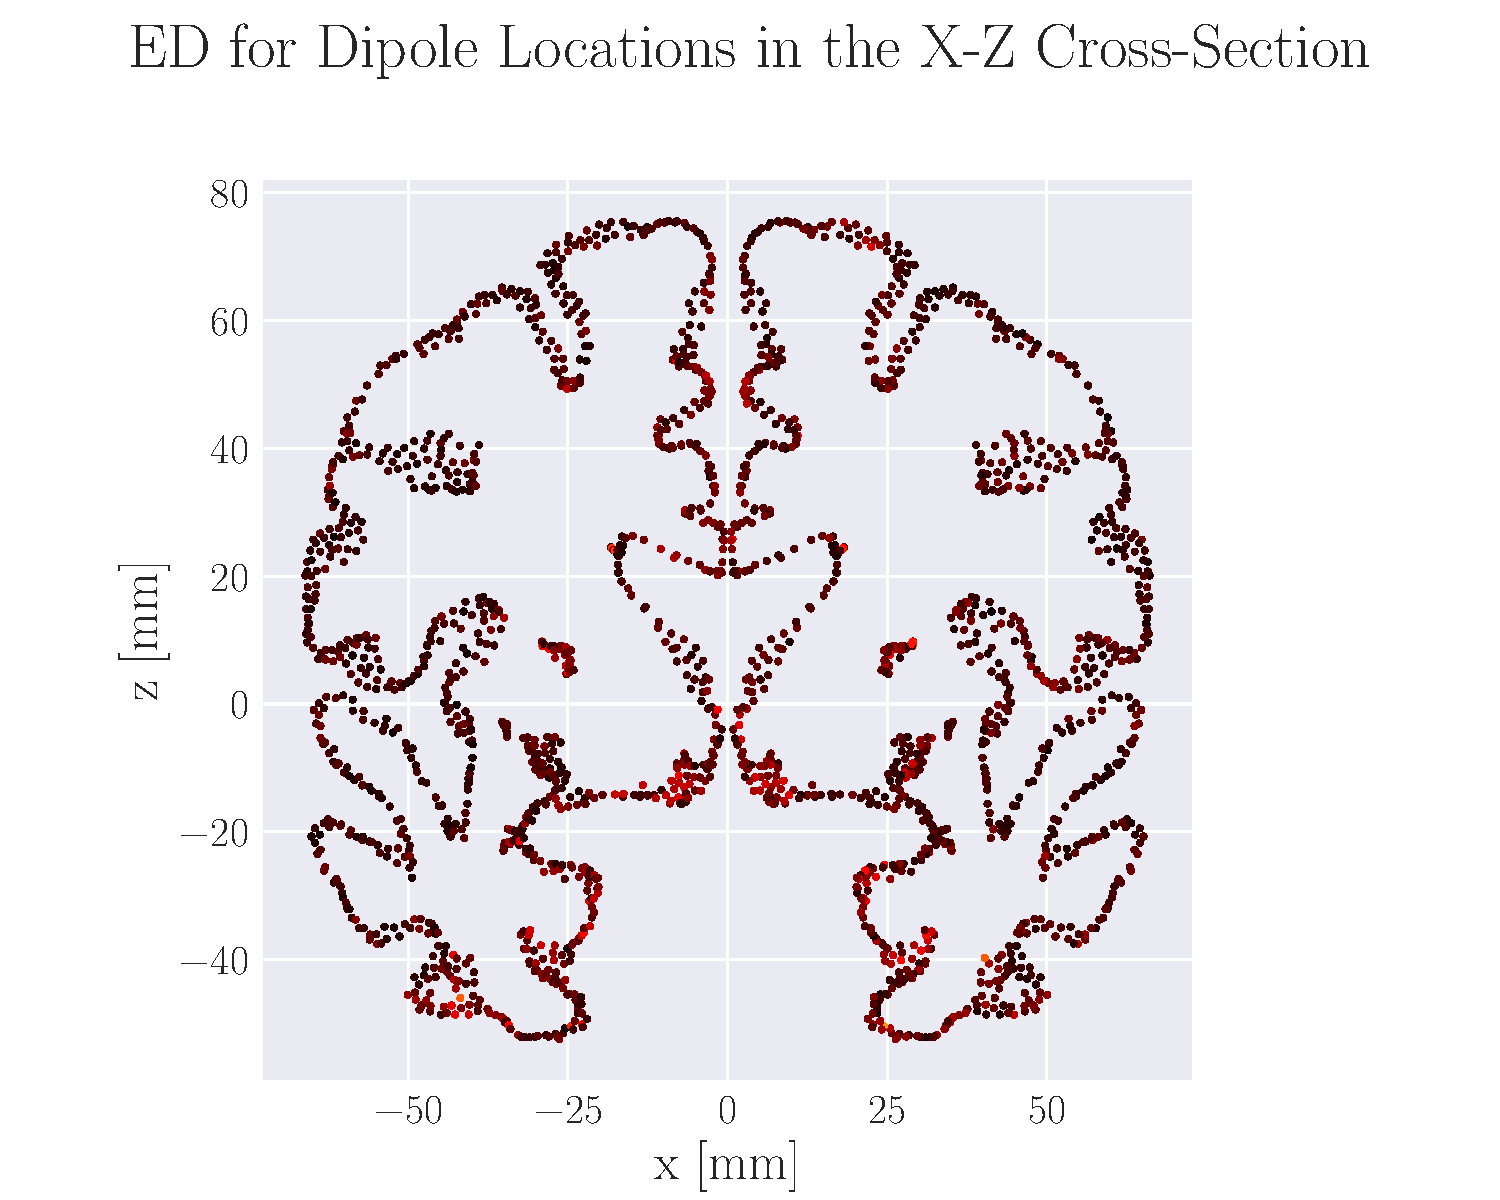
\includegraphics[width=0.7\linewidth]{figures/simple/MED_simple_dipole_error_Euclidean Distance_0.pdf}
    \vspace{10pt} % Adjust the vertical spacing between the images
    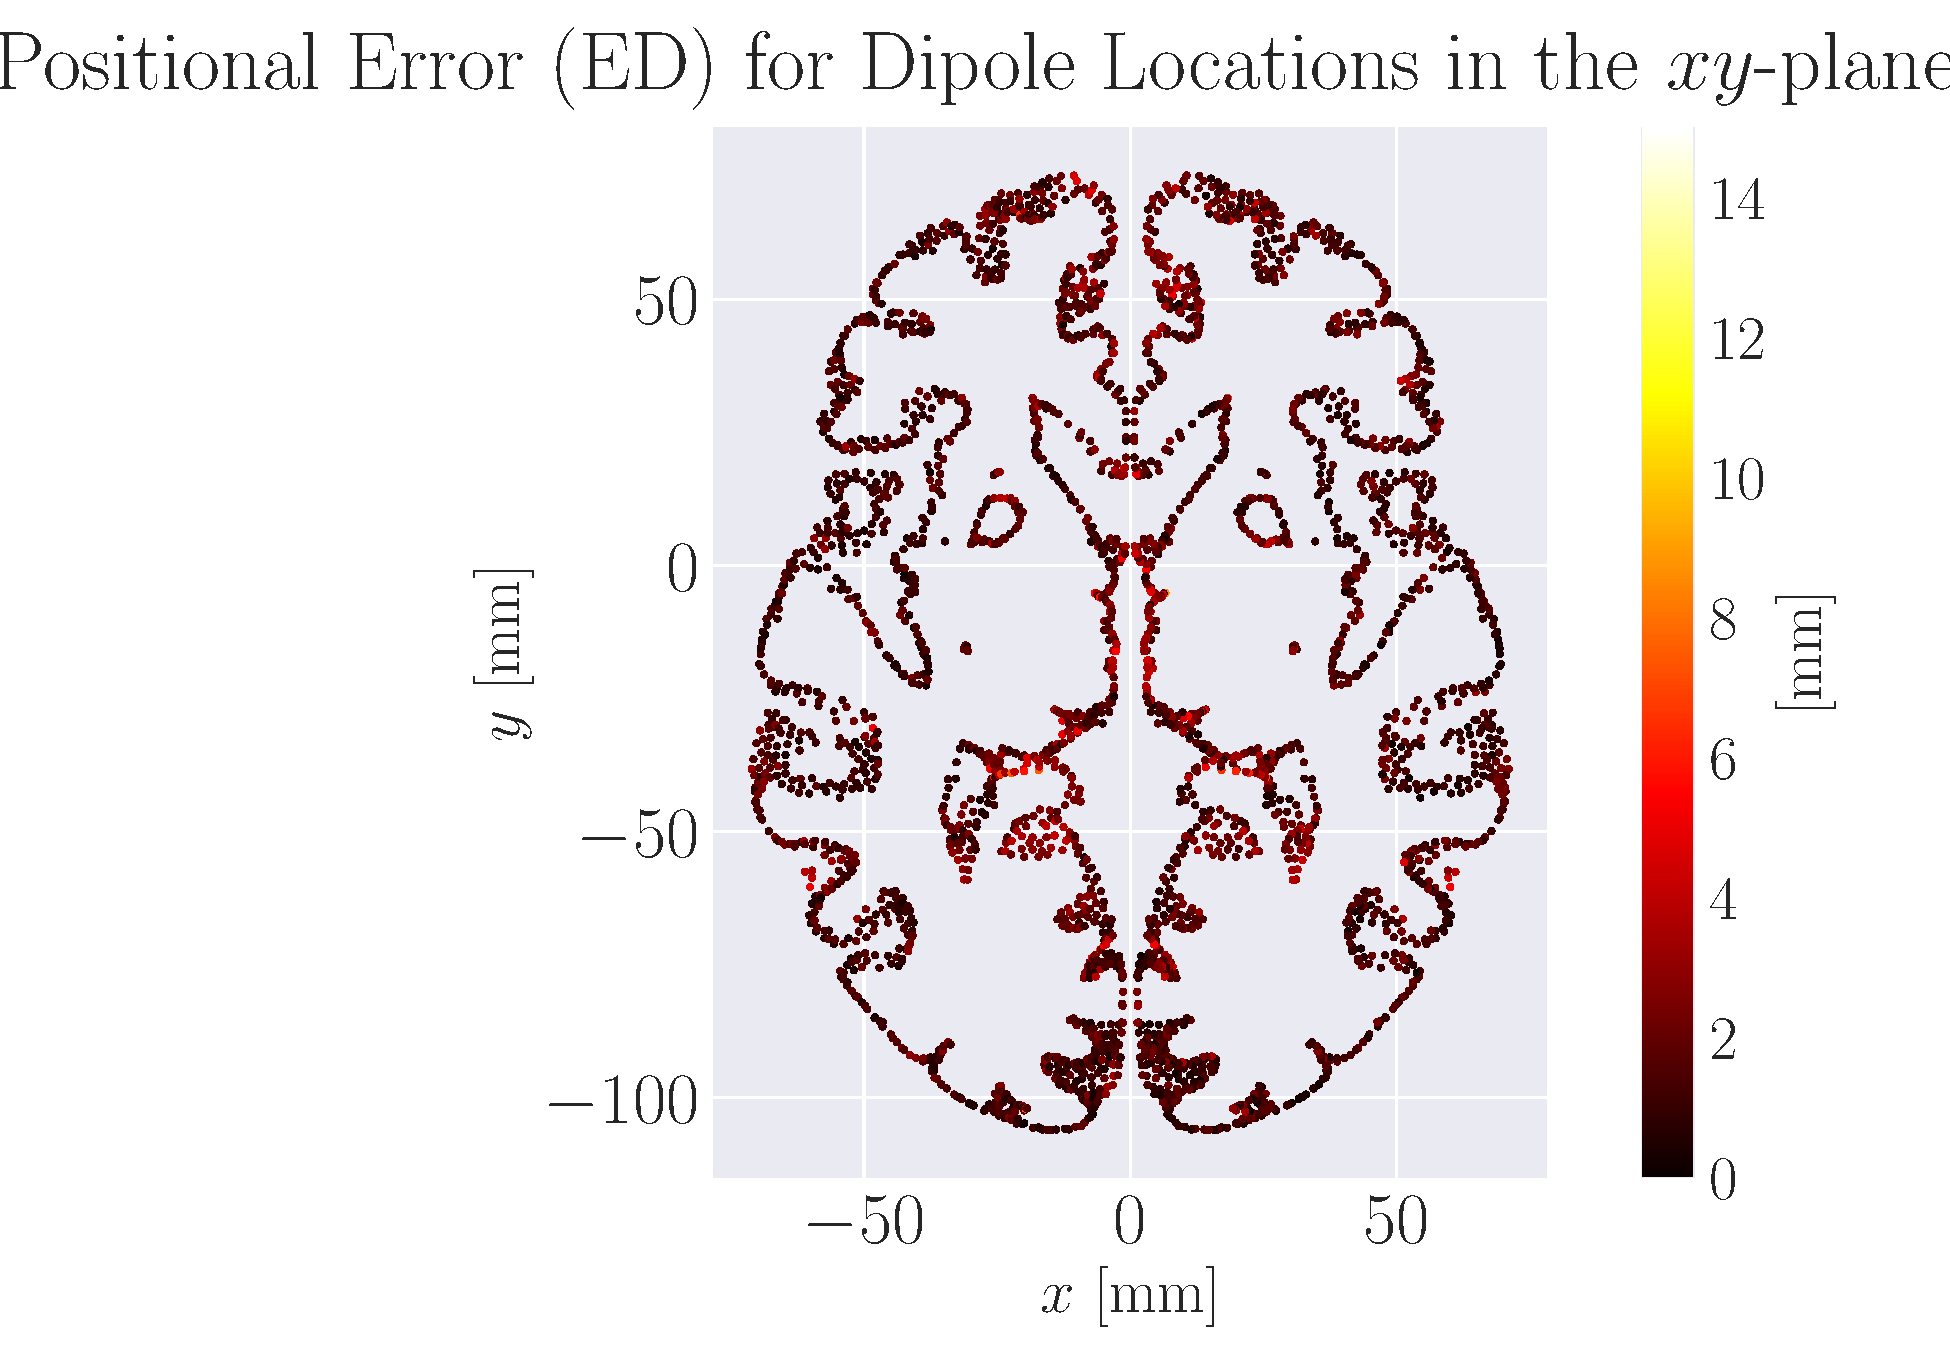
\includegraphics[width=0.7\linewidth]{figures/simple/MED_simple_dipole_error_Euclidean Distance_1.pdf}
    \vspace{10pt} % Adjust the vertical spacing between the images
    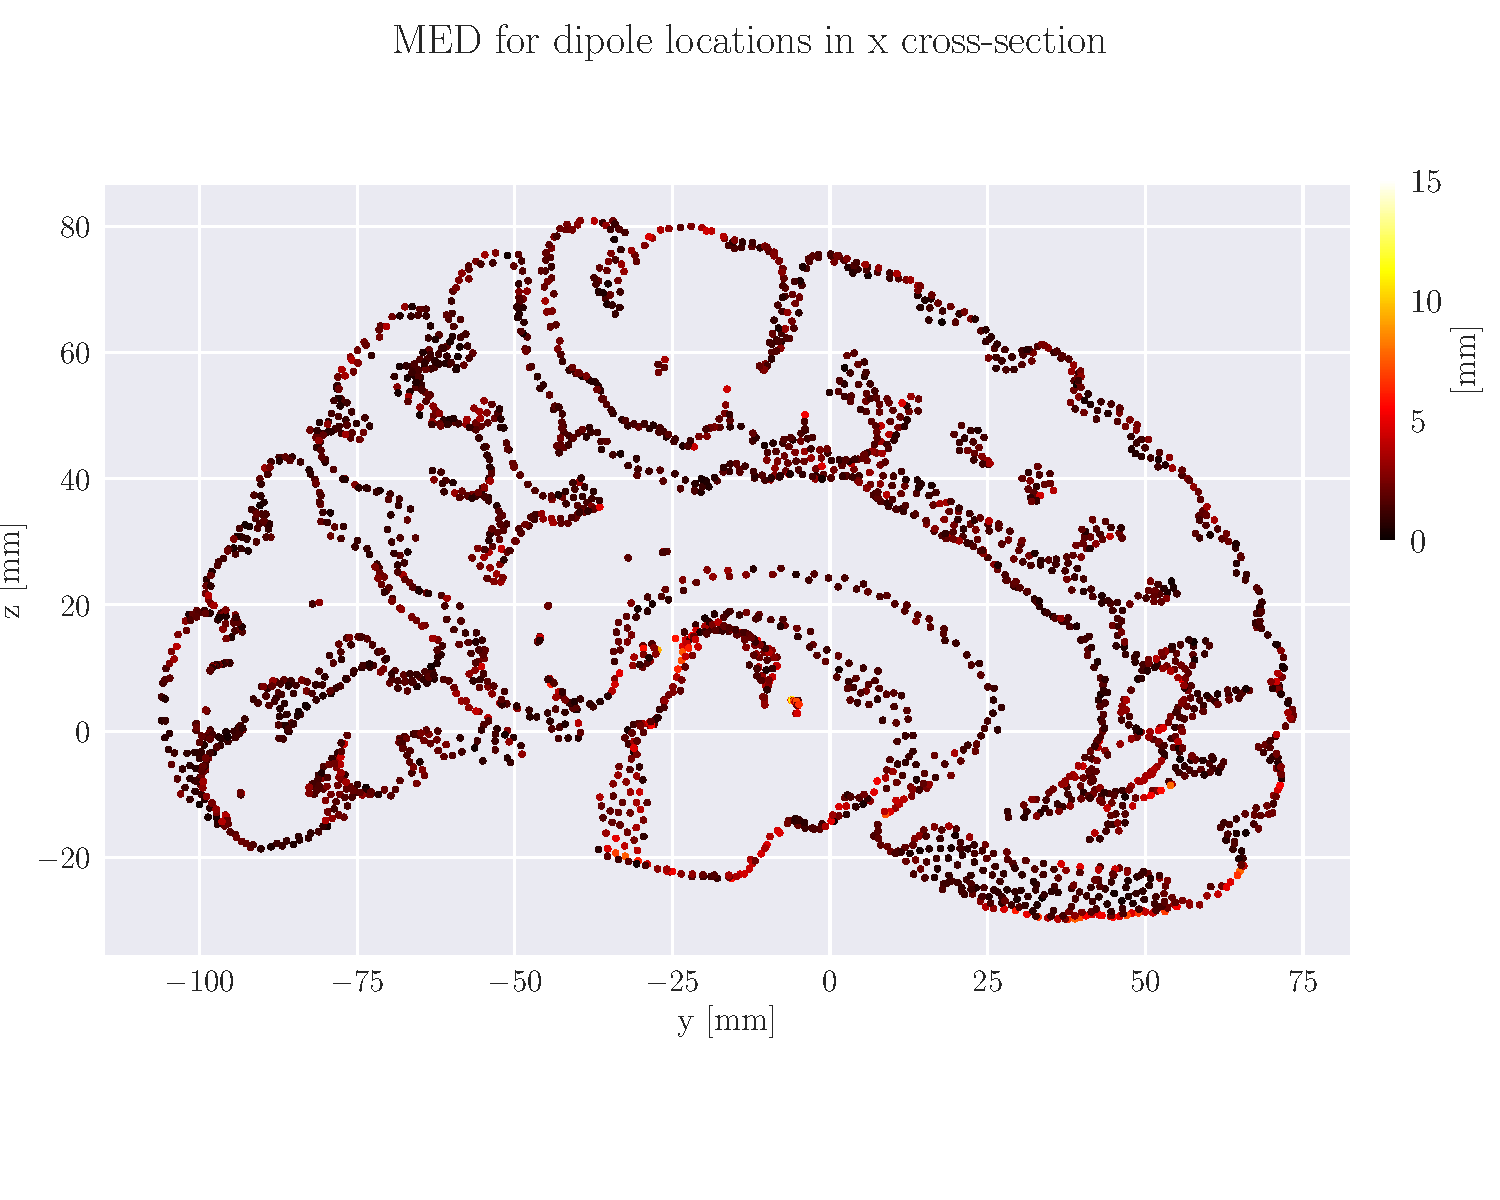
\includegraphics[width=0.7\linewidth]{figures/simple/MED_simple_dipole_error_Euclidean Distance_2.pdf}
    \caption{Different cross-sections of the cortex from the New York head model, seen from front, top and side. Each scatter point represents a possible position in the cortex matrix. The color of the fill in each circle indicates the Eucledian distance (ED) between the prediction and true value for the position of the specific dipole.}
    \label{fig:MED_crossections}
\end{figure}



\end{document}
